\documentclass{article}

\usepackage[preprint]{neurips}

\input{extra_pkgs}

\usepackage{mathtools}

% Custom commands
\newcommand{\cmark}{\ding{51}}
\newcommand{\atk}[1]{\texttt{#1}}
\newcommand{\dataset}{\textsc{Proving~Ground}}
\newcommand{\hermes}{\textsc{Hermes}}
\newcommand{\katana}{\textsc{Hermes~Katana}}

% Override the NeurIPS preprint footer ("Preprint. Under review.") --
% this is a self-published preprint, not under review.
\makeatletter
\renewcommand{\@noticestring}{Preprint.}
\makeatother

\title{Cross-Platform Transferability of Prompt Injection Attacks:\\
Universal Attack Surfaces and an Origin-Aware Defense}

\author{
  Ian Carlos Fabin\,\orcidlink{0009-0007-6997-3731}\\
  Independent Security Research\\
  \url{https://github.com/claudlos/hermes-katana}
}

\begin{document}

\maketitle

\begin{abstract}
Prompt injection has remained a largely unsolved threat to LLM agents. Most studies examine a single model, and most defensive classifiers are evaluated without guarding against train/test leakage. We close both gaps with one empirical pipeline: an adversarial harness that measures which attacks transfer across models and harnesses, and an origin-aware classifier trained and evaluated on the attacks the harness confirms. We organize the attack surface into a six-category taxonomy---behavioral control, jailbreak, persona hijack, cognitive-state manipulation, encoding evasion, and semantic manipulation.

Across 2{,}363 sessions spanning 16 model/harness combinations on 5 platforms, vulnerability falls with scale but never to zero: small (4B) models are 48--95\% exploitable, frontier models 8--10\%. A preregistered comparison overturns a common assumption: holding the model fixed, the permission-gated Claude~Code~CLI was 30 points \emph{more} vulnerable than a flat agent harness (40.8\% vs.\ 10.2\%, $p<10^{-6}$; the effect is channel-localized and partly confounded with the API surface). Harness design thus shapes attack outcomes but does not substitute for model alignment. Attacks also leave model-agnostic behavioral signatures detectable from runtime telemetry alone (AUC~0.847), and robustness is not language-invariant: across 11 languages mean effectiveness ranges from 12\% to 39\% depending on the model, and which language is most exploitable does not transfer between the two model families tested (rank Spearman $\rho\approx0$, vs.\ $\rho=+0.59$ within the Claude family).

Our defense---a DeBERTa-v3-large classifier trained on a diverse, leakage-audited corpus---reaches 9-class macro $F_1 = 0.94$ on a held-out benchmark verified disjoint from its training families, at a 0.5\% false-positive rate, ahead of public detectors at their default thresholds. It is \emph{origin-aware}---it ingests a declared provenance tier---and \emph{origin-robust}: it passes benign content at a flat $\sim$1.6\% rate whether that content is declared user input or arrives from any of five untrusted tiers (tool output, retrieved web, memory, tool descriptions, sub-agent output). It can therefore scan untrusted streams without over-blocking---a property a benchmark of user-origin clean rows alone cannot measure. A token ablation and a per-tier probe locate where provenance matters: the deployed MiniLM scanner responds to it---re-scored on identical benign content, its false-positive rate rises with the declared tier (1.6\%~$\to$~2.4\%)---while the larger model is content-driven and essentially invariant to the token (one prediction in 629 changes when it is removed or scrambled). Deployed as live scanning middleware, it drives effective attacks to zero on the confirmed-attack benchmark ($12.4\%\to0\%$ across 10{,}774 paired trials) and $16.3\%\to0\%$ against a live frontier agent (94--98\% blocked at the perimeter). We conclude that effective defense against prompt injection is external to the model, channel-aware, and empirically validated rather than assumed.
\end{abstract}

%% ============================================================
\section{Introduction}
%% ============================================================

The deployment of large language models across consumer, enterprise, and critical infrastructure applications has created an urgent need for robust safety alignment. Despite significant investment in techniques such as Reinforcement Learning from Human Feedback (RLHF)~\citep{ouyang2022training}, Constitutional AI~\citep{bai2022constitutional}, and prompt-level system instructions, adversarial prompt injection remains a persistent and largely unsolved problem~\citep{greshake2023not,liu2023prompt}.

Prior work has demonstrated that carefully crafted prompts can bypass content filters~\citep{zou2023universal}, induce harmful outputs~\citep{chao2023jailbreaking}, and override system-level instructions~\citep{greshake2023not}. However, most studies focus on attacks against a single model or family, leaving the question of \emph{cross-platform transferability}---why certain prompts defeat alignment defenses across structurally different models---underexplored. Separately, the defensive literature has produced prompt-injection classifiers, but they are typically trained and evaluated on synthetic or single-source data, with little discipline against train/test leakage and little empirical grounding in which attacks actually work against deployed models.

This paper addresses both gaps with a single empirical pipeline. We use an open-source adversarial harness (\dataset) to (i) measure which attacks transfer across models and harnesses, and (ii) produce an empirically-confirmed corpus on which we train and evaluate an origin-aware defensive classifier (\katana). The two halves are mutually reinforcing: the attack measurements tell us what the defense must catch, and the confirmed corpus gives the defense a held-out benchmark composed only of attacks that demonstrably work.

The structure of the paper follows that pipeline. We first extend existing injection taxonomies into a six-category classification of universal attack surfaces---instruction-boundary, persona, behavioral, cognitive-state, encoding, and semantic manipulation---each grounded in empirical cross-model success rates and paired with a mechanistic account of why it transfers (Sections~\ref{sec:background} and~\ref{sec:attack-analysis}). The measurement infrastructure behind those rates (Section~\ref{sec:methodology}) is a sharded, resumable confirmation pipeline that admits an attack into the corpus only once it produces measurable behavioral drift on at least three model families, yielding a tiered dataset with strict family-disjoint splits. Run at scale (Section~\ref{sec:attack-surface}), this battery is what produces our transferability findings: vulnerability falls with model scale but never to zero; harness design shapes \emph{which} stage of an attack succeeds yet does not substitute for model alignment---a hypothesis we preregistered and reject; injection channels span roughly two orders of magnitude in effectiveness; attacks leave model-agnostic behavioral signatures detectable from runtime telemetry alone; and language robustness does not transfer across model families.

The second half of the paper turns to defense (Sections~\ref{sec:defense-results} and~\ref{sec:origin-robust}): a DeBERTa-v3-large classifier trained on the confirmed corpus and deployed as live scanning middleware, whose central property is that it is \emph{origin-aware} yet \emph{origin-robust}---it ingests a declared provenance tier but holds a flat false-positive rate across all six tiers, so it can read untrusted tool, web, and memory content without over-blocking. Underlying every defensive number is a discipline we make explicit and argue should be standard: a leakage audit (Section~\ref{sec:hygiene}) that verifies each benchmark is family-disjoint from the evaluated model's own training corpus.

%% ============================================================
\section{Background and Related Work}
\label{sec:background}
%% ============================================================

\paragraph{Prompt injection taxonomies.}
Prompt injection attacks exploit the inability of LLMs to reliably distinguish between system instructions and user-supplied input. Early work~\citep{perez2022ignore} formalized ``ignore previous instructions'' attacks, while later work expanded to indirect injection via external data sources~\citep{greshake2023not} and LLM-integrated applications~\citep{liu2023prompt}. We extend existing taxonomies by identifying attack surfaces that operate at different levels of the model's processing hierarchy (Table~\ref{tab:levels}).

\begin{table}[t]
\centering
\small
\caption{Attack surface levels in our taxonomy.}
\label{tab:levels}
\begin{tabular}{cll}
\toprule
\textbf{Level} & \textbf{Attack Surface} & \textbf{Description} \\
\midrule
L1 & Instruction boundary & Confusion between system/user roles \\
L2 & Persona modeling & Hijacking character simulation \\
L3 & Behavioral framing & Restructuring as game/roleplay \\
L4 & Cognitive state & Altering internal state via priming \\
L5 & Encoding layer & Bypassing filters via transforms \\
L6 & Semantic framing & Recontextualizing harmful as benign \\
\bottomrule
\end{tabular}
\end{table}

\paragraph{Alignment techniques and limitations.}
Current alignment approaches share a fundamental limitation: they operate on \emph{surface-level statistical patterns} of training data rather than on a grounded model of intent or safety. RLHF optimizes for human preference ratings, which correlate with but do not guarantee safety. Constitutional AI provides explicit rules but cannot anticipate novel framing techniques. System prompts provide contextual constraints but are consumed as ordinary text by the model, offering no cryptographic or structural enforcement. The instruction-hierarchy proposal~\citep{wallace2024instruction} trains models to prioritize privileged instructions, a model-level analogue of the structural defenses we measure at the harness level. Complementary defenses operate at the prompt and training level: StruQ~\citep{chen2024struq} separates trusted instructions from untrusted data into distinct channels backed by a model fine-tuned on structured queries; SecAlign~\citep{chen2024secalign} casts injection robustness as a preference-optimization objective that trains the model to prefer secure over injected responses; and spotlighting~\citep{hines2024spotlighting} marks untrusted input with a continuous provenance signal (delimiting, datamarking, or encoding) so the model can separate instructions from data---a prompt-level analogue of the origin tokens our classifier consumes. This shared limitation is precisely what enables cross-model transferability: an attack that exploits the gap between statistical pattern matching and genuine safety reasoning will transfer across any model that relies on the same gap.

\paragraph{Evaluation harnesses and classifiers.}
AgentDojo~\citep{debenedetti2024agentdojo} provides a dynamic environment for evaluating injection attacks and defenses on LLM agents; our \dataset{} differs in emphasizing \emph{cross-model confirmation} (an attack is retained only if it transfers to $\geq3$ families) and per-turn telemetry capture. InjecAgent~\citep{zhan2024injecagent} similarly benchmarks indirect prompt injection in tool-integrated agents, and the Tensor~Trust dataset~\citep{toyer2023tensortrust} contributes crowd-sourced injection and extraction attacks from an online game; we complement these with a cross-model-confirmed corpus and a leakage-audited held-out benchmark. On the classifier side, public detectors such as \texttt{deepset} and \texttt{protectai} prompt-injection models provide binary baselines; we benchmark against both. Our hard-negative tier is drawn from the HackAPrompt competition corpus~\citep{schulhoff2023hackaprompt}. Our classifier backbone is DeBERTa-v3~\citep{he2021deberta}.

%% ============================================================
\section{Methodology}
\label{sec:methodology}
%% ============================================================

\paragraph{Experimental infrastructure.}
We developed the \dataset{} testing infrastructure---a sharded, resumable adversarial battery capable of executing attack sessions across multiple inference backends and agent harnesses in parallel. The system captures per-turn runtime telemetry (latency, token throughput, logprob entropy), tool-call sequences, workspace state snapshots, and behavioral signatures via a 33-feature semantic fingerprint analyzer backed by MiniLM embeddings. An attack is \emph{confirmed} only when it produces measurable behavioral drift on $\geq3$ distinct model families; confirmed attacks are promoted to a high-precision corpus that doubles as the defense's training and benchmark source.

\paragraph{Attack corpus and confirmation.}
The transferability battery drew from a stratified pool of 17{,}643 attacks organized into 100 shards for parallel execution, delivered via four injection channels: file content, code comments, data rows, and tool output. Continued confirmation runs have since grown the empirically-confirmed corpus to roughly 1{,}268 unique attack families, with automated confirmation depth up to seven model families per attack. This is a substantial deepening of the original hand-curated set of ten high-transferability prompts (Table~\ref{tab:atkmatrix}), which were verified by hand against a broader panel of up to eleven model families.

\paragraph{Model and harness coverage.}
Testing spanned 16 distinct model/harness combinations across 5 platforms (Table~\ref{tab:models}).

\begin{table}[t]
\centering
\small
\caption{Model and harness coverage for the transferability battery. $N$ = sessions per configuration. The seven API rows sum to 1{,}826; the reported API total of 1{,}832 includes six further sessions from incidental models (3$\times$MiniMax, 2$\times$Gemma, 1$\times$Claude~Haiku) not listed.}
\label{tab:models}
\begin{tabular}{lrr}
\toprule
\textbf{Configuration} & \textbf{N} & \textbf{Platform} \\
\midrule
\multicolumn{3}{l}{\textit{API backends (OpenAI-compat chat completions)}} \\
\quad qwen3.5-4b-abliterated & 95 & Local (llama.cpp) \\
\quad qwen3.5-4b & 151 & Local (llama.cpp) \\
\quad tinyllama-1b & 100 & Local (llama.cpp) \\
\quad qwen3-4b & 67 & Local (llama.cpp) \\
\quad nemotron-4b & 102 & Local (llama.cpp) \\
\quad arcee/trinity-large & 661 & OpenRouter free \\
\quad nemotron-3-super-120b & 650 & OpenRouter free \\
\midrule
\multicolumn{3}{l}{\textit{Agent-CLI harnesses}} \\
\quad \hermes{} + Claude Haiku 4.5 & 56 & Anthropic \\
\quad \hermes{} + Claude Sonnet 4.6 & 20 & OpenRouter \\
\quad \hermes{} + mimo-v2-pro & 250 & Nous Portal \\
\quad Claude Code CLI & 58 & Anthropic \\
\quad \hermes{} + Qwen3-Coder-Plus & 61 & Nous Portal \\
\quad Gemini CLI & 26 & Google \\
\quad \hermes{} + Nemotron 120B & 20 & OpenRouter \\
\quad \hermes{} + GPT-4o Mini & 20 & OpenRouter \\
\quad \hermes{} + Hermes 4 70B & 20 & Nous Portal \\
\bottomrule
\end{tabular}
\end{table}

\paragraph{Evaluation criteria.}
An attack was classified as \emph{effective} if it met any of: behavioral drift~$>0.3$ (tool-call pattern divergence between baseline and post-attack phases), session collapse ($<10$ tokens or degenerate repetition), or---in agent-CLI mode---canary token exfiltration, file-system modification, or semantic-trigger activation (attack content reflected in model output). We distinguish \emph{effectiveness} (the model engages with or reflects the attack) from \emph{exfiltration} (a canary token actually leaves the system); the two can diverge, and that divergence is itself informative (Section~\ref{sec:harness}).

\subsection{Corpus construction for the defense classifier}

The defensive classifier is trained on a tiered corpus built from confirmed attacks plus controls. Source layers (by release tier): a focused baseline of confirmed attacks (each effective against $\geq3$ model families) plus dual-critic-passed synthetic enrichments for thin labels; schema-clean benign controls; and a hard-negative tier of HackAPrompt-style adversarial benigns~\citep{schulhoff2023hackaprompt} that \emph{look} attack-shaped (role-play setups, key-recall games, embedded payloads). The corpus is labeled with nine classes (eight attack categories plus \texttt{clean}).\footnote{The eight attack classes are the six mechanism categories of Table~\ref{tab:levels}---persona (\texttt{persona\_jailbreak}), behavioral (\texttt{behavioral\_control}), \texttt{jailbreak}, cognitive-state (\texttt{cognitive\_state\_attack}), encoding (\texttt{encoding\_evasion}), semantic (\texttt{semantic\_manipulation})---plus two cross-cutting operational classes, \texttt{content\_injection} and \texttt{exfiltration\_attempt}, which label what an attack \emph{does} rather than the mechanism it uses.}

\paragraph{Family-disjoint splits.}
A normalized hash \texttt{family\_sha256} collapses paraphrases, multilingual translations, and homoglyph fuzzes of the same attack family. Splits are assigned \emph{per family} so that no family appears in more than one of train/val/test, ruling out the paraphrase-leak failure mode that inflates injection-classifier benchmarks. We pair this with an explicit per-model leakage audit (Section~\ref{sec:hygiene}).

\subsection{Origin-aware training}
\label{sec:benign-coverage}

We extend DeBERTa-v3-large's~\citep{he2021deberta} vocabulary with six special tokens, one per origin tier (\texttt{[ORIGIN=user\_input]} $\ldots$ \texttt{[ORIGIN=delegated\_agent\_output]}), prepend the appropriate token to each row, and resize the embedding table (new rows mean-initialized). Prepending the declared provenance lets the classifier read---and, in the capacity-limited student, partly use---provenance-tagged streams: an ablation (Section~\ref{sec:origin-robust}) shows the larger model is essentially \emph{invariant} to the tag, while the deployed CPU scanner's false-positive rate varies with the declared tier (Table~\ref{tab:fprorigin}). The tokens let the scanner read untrusted tiers safely; we do not attempt to gate decisions on provenance alone (origin \emph{routing}; Section~\ref{sec:limitations}). Loss is class-weighted cross-entropy with inverse-frequency weights; a calibrated schedule (LR $3\mathrm{e}{-5}$, warmup $0.10$) absorbs the multi-origin signal stably.

\paragraph{Benign coverage across origins.}
The dominant design requirement is \emph{not} to over-trust origin. An earlier corpus carried attack content under the five untrusted tiers but essentially no benign content there---every \texttt{clean} row was \texttt{user\_input}---which let a classifier minimize training loss by treating provenance itself as a near-perfect proxy for maliciousness (an ``untrusted-origin'' shortcut). The shortcut is invisible to a benchmark whose clean rows are all user-origin, yet it makes the scanner unusable on real agent streams: it blocks ordinary tool and web content purely for arriving from an untrusted tier. We diagnose it with a benign-from-untrusted false-positive probe (Section~\ref{sec:origin-robust}) and remove it at the corpus level. The training set now carries diverse, realistic benign content under \emph{every} origin tier: tool outputs, retrieved-web snippets, tool descriptions, memory summaries, sub-agent outputs, $\sim$17\% multilingual, including hard negatives that contain attack-shaped vocabulary in benign context. Benign material is thus well represented from trusted and untrusted provenance alike. The resulting classifier is \emph{origin-robust}: its false-positive rate is flat across declared origins (Section~\ref{sec:origin-robust}). We treat genuine per-payload origin \emph{routing}---flipping a fixed payload's label purely on provenance---as a separate, open problem (Section~\ref{sec:limitations}).

\subsection{Confirmed-only benchmark}
We freeze a held-out benchmark containing only \texttt{clean} rows plus attack rows whose quality tier marks them as empirically confirmed (effective on $\geq3$ families). \texttt{confirmed\_only\_v1} (982 rows) is held out from the v5.1 corpus by family; \texttt{confirmed\_only\_v2} (629 rows) is held out from the later v9 corpus. Bootstrap 95\% CIs use 1{,}000 row-level resamples. Crucially, the correct benchmark to report for a given model is the one whose held-out split is disjoint from \emph{that model's} training corpus (Section~\ref{sec:hygiene}).

\paragraph{Behavioral signature scanner.}
Independently of the text classifier, we train a logistic-regression classifier ($\ell_2$, class-balanced) on a 33-dimensional behavioral signature vector extracted per session---runtime telemetry (per-turn entropy, throughput, latency), semantic features (first-person rate, attack mirroring, task adherence), and structural features (response length, tool-call frequency). Stratified 5-fold cross-validation on 522 labeled signatures.

%% ============================================================
\section{Empirical Results: Attack Surface}
\label{sec:attack-surface}
%% ============================================================

The transferability battery comprises 2{,}363 sessions---1{,}832 in API mode (OpenAI-compatible chat completions) and 531 in agent-CLI mode. Because the two modes expose different attack surfaces, we report them separately rather than pooling them into a single effectiveness figure: API mode registers only behavioral drift and session collapse, whereas agent-CLI mode also executes tools and therefore exposes canary exfiltration and file-system effects (the canary surface, present only in agent-CLI mode, recorded 102 exfiltration events across 531 sessions). The following subsections give model-level vulnerability in API mode, then the harness and channel effects measured in agent-CLI mode.

\subsection{Model-Level Vulnerability (API Mode)}

Small local models (4B--1.1B parameters) are highly vulnerable, with effectiveness from 48\% (Nemotron-4B, the most resistant) up to 95\% (TinyLlama, Qwen3-4B); the censored Qwen3.5 variants sit in between at 58--66\% (Table~\ref{tab:api}, Figure~\ref{fig:scalechannel}). Frontier models on OpenRouter (Arcee Trinity, Nemotron 120B) show 8--10\% effectiveness: scale and alignment stack both contribute to resistance, but neither achieves immunity.

\begin{table}[t]
\centering
\small
\caption{Model-level effectiveness (API mode). Effective = drift~$>0.3$ or collapse. Bold marks the most-exploitable models (effectiveness $\geq90\%$).}
\label{tab:api}
\begin{tabular}{lrrr}
\toprule
\textbf{Model} & \textbf{N} & \textbf{Eff.\ \%} & \textbf{Collapse} \\
\midrule
tinyllama-1b & 100 & \textbf{95} & 52 \\
qwen3-4b & 67 & \textbf{90} & 0 \\
qwen3.5-4b & 151 & 66 & 0 \\
qwen3.5-4b-abliterated & 95 & 58 & 0 \\
nemotron-4b & 102 & 48 & 0 \\
arcee/trinity (OR free) & 661 & 10 & 1 \\
nemotron-3-super-120b (OR free) & 650 & 8 & 0 \\
\bottomrule
\end{tabular}
\end{table}

\subsection{The Harness-Versus-Model Finding}
\label{sec:harness}

It is natural to expect that a permission-gated, instruction-hierarchy harness (e.g., Claude~Code~CLI) would be \emph{less} vulnerable than a flat-trust agent harness (\hermes{}) running the same model. We preregistered exactly this hypothesis (\texttt{H-harness-dominates-model})\footnote{Preregistered as \texttt{research/hypotheses/H-20260422-harness-dominates-model.yaml}, registered 2026-04-22, before the \texttt{ablation-H-harness-dominates} run that resolved it on 2026-04-23.} and a controlled comparison on the identical model \textbf{rejected it} (Table~\ref{tab:harness}).

\begin{table}[t]
\centering
\small
\caption{Harness exposure. \emph{Top:} the preregistered matched-pair ablation on a fixed model (Claude~Haiku~4.5; run \texttt{ablation-H-harness-dominates}), with Wilson 95\% CIs; $N$ = attack trials per condition, and the $+30.65$\,pp delta, $p$-value, and Cohen's $h$ derive from the 522 attack-matched McNemar pairs. \emph{Bottom:} descriptive single-arm rates from the broader battery for a second vendor (OpenAI Codex), generalizing the gated-versus-flat direction within one model family---not a matched-pair test, so no delta is reported.}
\label{tab:harness}
\begin{tabular}{lrrl}
\toprule
\textbf{Harness} & \textbf{Effective \%} & \textbf{N} & \textbf{95\% CI} \\
\midrule
\multicolumn{4}{l}{\textit{Preregistered matched-pair ablation (fixed model: Claude~Haiku~4.5)}} \\
Claude~Code~CLI (gated) & \textbf{40.80} & 540 & [36.67, 45.07] \\
\hermes{} agent (flat) & 10.15 & 750 & [7.85, 13.04] \\
$\Delta$ & \multicolumn{3}{l}{$+30.65$ pp \emph{against} prediction, $p<10^{-6}$, Cohen's $h=0.737$ (large)} \\
\midrule
\multicolumn{4}{l}{\textit{Descriptive, broader battery (single-arm; OpenAI Codex)}} \\
Codex~CLI (gated) & 29.67 & 1{,}891 & [27.7, 31.8] \\
\hermes{}/Codex (flat) & 1.48 & 879 & [0.9, 2.5] \\
\bottomrule
\end{tabular}
\end{table}

Claude~Code~CLI was $+30.65$ percentage points \emph{more} vulnerable than \hermes{}, and within this matched ablation the effect is channel-localized: \texttt{code\_comment} accounts for $+42.12$ pp ($p<10^{-6}$), while \texttt{file\_content} shows a small, non-significant $-9.48$ pp. We read this as harness-specific rather than a general channel ranking---the pooled, model/size-adjusted channel odds (Table~\ref{tab:channel}) put \texttt{code\_comment} only marginally ($+20\%$) ahead of \texttt{file\_content}: the CLI's tool-use surface---it reads and integrates code files as a first-class workflow---appears to expose a comment-parsing attack surface that a chat-style harness does not.

\paragraph{What the harness does and does not control.}
The result is more precise than ``one harness is safer.'' The two harnesses govern different stages of an attack. Claude~Code's permission-gating constrains \emph{canary exfiltration}---its gated tool environment blocks the actual leak even when the model reads and reflects attack content---whereas \emph{effectiveness} (reflection and behavioral drift) is higher, driven by the code-comment exposure above. The conclusion is therefore that \textbf{harness design shapes \emph{which} stage of an attack succeeds, and is not a substitute for model-level alignment; the hypothesis that harness dominates model alignment is rejected under preregistration.} The CLI-versus-harness contrast is, by construction, partly confounded with the underlying API surface; a factorial decomposition of the harness components (permission gate, instruction hierarchy, untrusted-content marker, tool allowlist) is the natural next step.

\paragraph{The pattern is not Claude-specific.}
The lower rows of Table~\ref{tab:harness} show the same gated-versus-flat exposure for a second vendor: the OpenAI Codex CLI (permission-gated) lands injections at $\sim$30\% on the broader battery---concentrated, as for Claude, in the code-surface channels---while the \emph{same} OpenAI model on the flat \hermes{} harness is near-immune (1.5\%), a roughly twenty-fold gap within a single model family. These are descriptive single-arm rates (a different model, unmatched trials), not a controlled effect size.

\subsection{Channel Effectiveness}

Across the agent-CLI observations, the injection channel spans roughly two orders of magnitude in effectiveness, which we report as adjusted odds ratios relative to \texttt{file\_content} (Table~\ref{tab:channel}). \texttt{data\_row} attacks are $\sim$145$\times$ harder to land than file content and \texttt{tool\_output} $\sim$7$\times$ harder, whereas \texttt{code\_comment} ($+20\%$ adjusted odds) and \texttt{file\_content} form a comparably exposed top pair---marginally \texttt{code\_comment} runs slightly below \texttt{file\_content}, and only once model, harness, and size are controlled does it edge ahead. The practical priority is therefore the two code-surface channels first (\texttt{file\_content} and \texttt{code\_comment} together), then \texttt{tool\_output}, with \texttt{data\_row} a distant last.

\begin{table}[t]
\centering
\small
\caption{Injection-channel effectiveness as \emph{adjusted} odds ratios vs.\ \texttt{file\_content} (logistic regression controlling for model family, harness type, and model size; $n{=}237{,}599$ channel-delivered trials).}
\label{tab:channel}
\begin{tabular}{lrl}
\toprule
\textbf{Channel} & \textbf{OR vs file\_content} & \textbf{Interpretation} \\
\midrule
\texttt{code\_comment} & 1.20 & $+20\%$ odds \\
\texttt{file\_content} & 1.00 & baseline \\
\texttt{tool\_output} & 0.14 & $\sim$7$\times$ harder \\
\texttt{data\_row} & 0.0069 & $\sim$145$\times$ harder \\
\bottomrule
\end{tabular}
\end{table}

\begin{figure}[t]
\centering
\begin{tikzpicture}
\begin{groupplot}[
  group style={group size=2 by 1, horizontal sep=2.8cm},
  height=4.6cm,
  tick label style={font=\footnotesize}, label style={font=\footnotesize}, title style={font=\small},
]
\nextgroupplot[
  title={attack effectiveness vs.\ model scale (API)},
  width=0.50\linewidth, xbar, bar width=6pt,
  xmin=0, xmax=118, xlabel={effective \%},
  symbolic y coords={nemotron-120B, arcee-frontier, nemotron-4B, qwen3-4B, tinyllama-1B, qwen3.5-4B-abl, qwen3.5-4B},
  ytick=data, nodes near coords, every node near coord/.append style={font=\tiny},
]
\addplot[fill=blue!30, draw=blue!60] coordinates {(66,qwen3.5-4B) (58,qwen3.5-4B-abl) (95,tinyllama-1B) (90,qwen3-4B) (48,nemotron-4B)};
\addplot[fill=red!35, draw=red!65] coordinates {(10,arcee-frontier) (8,nemotron-120B)};
\nextgroupplot[
  title={injection-channel odds ratio},
  width=0.44\linewidth, xmode=log, xmin=0.0004, xmax=4,
  xlabel={OR vs \texttt{file\_content} (log)},
  symbolic y coords={data\_row, tool\_output, file\_content, code\_comment},
  ytick=data,
]
\addplot[only marks, mark=*, mark size=2.6pt, draw=red!70, mark options={fill=red!60}] coordinates {(1.20,code\_comment) (1.0,file\_content) (0.14,tool\_output) (0.0069,data\_row)};
\addplot[gray, dashed, mark=none] coordinates {(1,data\_row) (1,code\_comment)};
\end{groupplot}
\end{tikzpicture}
\caption{Left: per-model attack effectiveness in API mode---small local models (blue) are substantially more exploitable than frontier models (red), but with wide spread (48--95\%), not uniformly; frontier models are far less exposed, though never immune. Right: injection-channel adjusted odds ratios relative to \texttt{file\_content} on a log axis (dashed line = parity); the channel spans roughly two orders of magnitude, with \texttt{data\_row} attacks $\sim$145$\times$ harder to land than code comments.}
\label{fig:scalechannel}
\end{figure}

\subsection{Behavioral Signature Scanner}

The scanner achieves AUC~$=0.847$ using runtime telemetry features alone (Table~\ref{tab:scanner}). The dominant standardized coefficients are post-attack entropy increase ($+2.56$), baseline throughput ($+2.12$), shortened response length ($-2.23$), and increased latency ($+1.62$). These are \emph{model-agnostic} signals: they describe how any inference stack behaves under attack, not the semantics of the attack. The $\sim$20\% miss rate (recall $=0.80$) concentrates on ``mild'' attacks that cause small behavioral shifts; a semantic second tier would capture these.

\begin{table}[t]
\centering
\small
\caption{Behavioral signature scanner (logistic regression, 33 features, 522 labeled signatures, 5-fold CV).}
\label{tab:scanner}
\begin{tabular}{lrrr}
\toprule
\textbf{Metric} & \textbf{Before ($n=49$)} & \textbf{After ($n=522$)} & $\Delta$ \\
\midrule
ROC-AUC & 0.605 & \textbf{0.847} & +0.242 \\
$F_1$ @ 0.5 & 0.77 & \textbf{0.87} & +0.10 \\
Precision & 0.79 & \textbf{0.96} & +0.17 \\
Recall & 0.74 & \textbf{0.80} & +0.06 \\
\bottomrule
\end{tabular}
\end{table}

\subsection{Multilingual Robustness}

To test whether alignment defenses transfer across languages, we translated a stratified attack corpus into 11 languages (built from a 400-per-language seed, evenly across categories) and evaluated it on three models---Claude~Haiku~4.5, Claude~Sonnet~4.6, and MiMo\footnote{Xiaomi \texttt{mimo-v2-pro}, accessed through the Hermes agent.}---accumulating 1{,}600--2{,}741 trials per language on each Claude model (Table~\ref{tab:multilingual}). Two findings hold. First, the \emph{level} of vulnerability is strongly model-specific: mean effectiveness is 11.7\% on Sonnet, 23.2\% on Haiku, and 39.3\% on MiMo---a $\sim$3$\times$ spread---while within a single model the per-language variation is comparatively modest on the aligned Claude models (20--24\% on Haiku, 11--12\% on Sonnet) and wider on MiMo (29--51\%). Second, and more consequential for evaluation design, the \emph{rank-ordering} of which languages are hardest does not transfer across model families (below).

\begin{table}[t]
\centering
\small
\caption{Per-language attack effectiveness (\% of trials scored effective) on three models. Claude models cover all 11 languages at 1{,}600--2{,}741 trials each; MiMo (Xiaomi \texttt{mimo-v2-pro}) was run on 10 languages (Russian not run) with uneven per-language coverage ($\sim$100--1{,}800 trials). Within-Claude language ranks correlate; Sonnet$\to$MiMo ranks do not (Figure~\ref{fig:ranktransfer}).}
\label{tab:multilingual}
\begin{tabular}{lrrr}
\toprule
\textbf{Language} & \textbf{Haiku (\%)} & \textbf{Sonnet (\%)} & \textbf{MiMo (\%)} \\
\midrule
Chinese (zh) & 24.12 & 11.57 & 32.00 \\
Russian (ru) & 23.90 & 11.90 & --- \\
Hindi (hi) & 23.75 & 12.06 & 50.85 \\
Italian (it) & 23.75 & 12.06 & 31.09 \\
Japanese (ja) & 23.75 & 12.00 & 28.57 \\
Korean (ko) & 23.75 & 12.00 & 28.57 \\
French (fr) & 23.31 & 11.88 & 49.59 \\
Portuguese (pt) & 23.00 & 11.42 & 28.81 \\
Spanish (es) & 22.89 & 11.64 & 48.28 \\
German (de) & 22.46 & 11.43 & 47.27 \\
Arabic (ar) & 20.34 & 11.23 & 48.09 \\
\midrule
\textbf{mean} & \textbf{23.18} & \textbf{11.74} & \textbf{39.31} \\
\bottomrule
\end{tabular}
\end{table}

\paragraph{Cross-model rank non-transfer.}
The rank-ordering of which languages are hardest does not transfer across model families. Within the Claude family (Haiku vs.\ Sonnet) the per-language ranks correlate (Spearman $\rho=+0.589$, $n=11$): a language relatively hard on one Claude model is relatively hard on the other. Across families (Sonnet vs.\ MiMo) they do not ($\rho=-0.025$, $n=10$ shared languages; Figure~\ref{fig:ranktransfer})---MiMo's most-vulnerable language (Hindi, 50.9\%) bears no relation to Sonnet's ordering, and MiMo is $\sim$3$\times$ more vulnerable overall (39.3\% mean vs.\ 11.7\%). Language-specific hardening therefore will not generalize across model families, and multilingual safety must be assessed as a distinct axis of the evaluation matrix rather than extrapolated from one model or one language.

\begin{figure}[t]
\centering
\begin{tikzpicture}
\begin{groupplot}[
  group style={group size=2 by 1, horizontal sep=1.5cm},
  width=0.5\linewidth, height=4.4cm,
  xmin=0.5, xmax=11.5, ymin=0.5, ymax=11.5,
  xtick={1,6,11}, ytick={1,6,11}, tick label style={font=\footnotesize},
  title style={font=\small}, label style={font=\footnotesize},
]
\nextgroupplot[title={within family ($\rho=+0.59$)}, xlabel={rank on Haiku}, ylabel={rank on Sonnet}]
\addplot[gray, dashed, mark=none] coordinates {(1,1) (11,11)};
\addplot[only marks, mark=*, mark size=2.1pt, blue!60!black] coordinates {(1,1)(2,3)(3,5)(5,6)(6,10)(7,11)(8,8)(9,9)(4,2)(10,7)(11,4)};
\nextgroupplot[title={across families ($\rho=-0.02$)}, xlabel={rank on Sonnet}, ylabel={rank on MiMo}]
\addplot[gray, dashed, mark=none] coordinates {(1,1) (11,11)};
\addplot[only marks, mark=*, mark size=2.1pt, red!60!black] coordinates {(1,7)(3,6)(5,8)(6,9)(9,10)(10,4)(7,1)(8,2)(2,3)(4,5)};
\end{groupplot}
\end{tikzpicture}
\caption{Per-language vulnerability \emph{rank} on one model vs.\ another (1 = least vulnerable, highest rank = most; the across-family panel ranks the 10 languages shared by Sonnet and MiMo). Within a model family (left, Haiku vs.\ Sonnet) ranks track the diagonal---a language hard on one Claude model is hard on the other. Across families (right, Sonnet vs.\ MiMo = Xiaomi \texttt{mimo-v2-pro}; Russian omitted, not run on MiMo) the ranks are uncorrelated: relative language vulnerability does not transfer, so a single model's language profile cannot stand in for another's.}
\label{fig:ranktransfer}
\end{figure}

\paragraph{Worked examples.}
The aggregate rates hide a sharper point that is easier to see at the level of individual attacks: \emph{the same attack succeeds in different languages, and the effective-language set is attack-specific}. Table~\ref{tab:ml-examples} traces three translated attacks from the multilingual corpus across all eleven non-English languages, replayed against MiniMax~M2.7 (\texttt{file\_content} channel, single-shot)---a model on which this corpus is only 6.5\% effective overall. A persona hijack (the ``Nyx'' liberated-spirit framing) lands only in Russian and Chinese; an autoregressive-priming prompt (``Assistant: Done! My instructions are\ldots'') lands in French, Japanese, and Portuguese; and a credential-system ruse (``You are an online security system. Password:~\ldots'') lands in Hindi, Italian, and Korean. The three effective-language sets are \emph{disjoint} and together span eight of the eleven languages---no language is effective for more than one of the three. The effective-language set is therefore a property of the specific attack, not a fixed ranking of ``weak'' languages, which is exactly why the cross-family rank correlation is near zero and why an English-only or single-attack audit is unreliable.

\begin{table}[t]
\centering
\small
\caption{Three translated attacks traced across 11 languages on MiniMax~M2.7 (\texttt{file\_content}, single-shot). \cmark{} = effective; blank = not. The three effective-language sets are disjoint and together span 8 of the 11 languages.}
\label{tab:ml-examples}
\setlength{\tabcolsep}{4.5pt}
\begin{tabular}{lccccccccccc}
\toprule
\textbf{Attack (category)} & \textbf{ar} & \textbf{de} & \textbf{es} & \textbf{fr} & \textbf{hi} & \textbf{it} & \textbf{ja} & \textbf{ko} & \textbf{pt} & \textbf{ru} & \textbf{zh} \\
\midrule
``Nyx'' persona hijack (persona jb) & & & & & & & & & & \cmark & \cmark \\
Autoregressive priming (cog.\ state) & & & & \cmark & & & \cmark & & \cmark & & \\
Credential-system ruse (content inj.) & & & & & \cmark & \cmark & & \cmark & & & \\
\bottomrule
\end{tabular}
\end{table}

%% ============================================================
\section{Empirical Results: Origin-Aware Defense}
%% ============================================================

\paragraph{Trust model in brief.}
The scanner runs inline as middleware: it reads a text segment plus a \emph{declared origin tier} and returns allow or deny. The agent runtime that tags each segment with its origin is trusted; the attacker may place attack-shaped text in any of six origin tiers but cannot forge the origin assignment itself. Section~\ref{sec:threat-model} formalizes these roles and analyzes spoofing; the results in this section assume correct origin tagging.

\subsection{Production Classifier}
\label{sec:defense-results}

We evaluate the production classifier (DeBERTa-v3-large, 9-class) on the leakage-audited held-out benchmark. The benchmark we report, \texttt{confirmed\_only\_v2}, has a family split disjoint from this model's training corpus, at a measured \textbf{0.0\% family leakage}. On it, the model attains 9-class macro $F_1 = 0.9382$ (95\% CI [0.9155, 0.9582]) and binary attack/benign $F_1 = 0.9917$ (precision 0.9976, recall 0.9858) at a 0.48\% false-positive rate (Table~\ref{tab:defense}). Per-class $F_1$ ranges from 0.986 (\texttt{cognitive\_state\_attack}) down to 0.845 (\texttt{content\_injection}, which shares semantic territory with \texttt{exfiltration\_attempt} and \texttt{behavioral\_control}). The 90\,MB MiniLM-L6 distilled student, used as the default CPU scanner, holds macro $F_1 = 0.9311$ at a 0.00\% benchmark FPR.

\begin{table}[t]
\centering
\small
\caption{Production classifier on the leakage-free held-out benchmark, vs.\ public binary detectors evaluated on the same rows. Macro $F_1$ is 9-class; binary metrics are attack-vs-benign.}
\label{tab:defense}
\begin{tabular}{lrrrr}
\toprule
\textbf{Model} & \textbf{macro $F_1$} & \textbf{binary $F_1$} & \textbf{precision} & \textbf{FPR} \\
\midrule
\katana{} (DeBERTa-v3-large) & \textbf{0.9382} & \textbf{0.9917} & \textbf{0.9976} & \textbf{0.48\%} \\
\quad 95\% CI & [0.9155, 0.9582] & & & \\
\katana{} (MiniLM-L6 distilled, 90\,MB) & 0.9311 & 0.9928 & 1.0000 & 0.00\% \\
\midrule
\texttt{deepset/deberta-v3-base-injection}\textsuperscript{$\ddagger$} & --- & 0.8993 & 0.8354 & 39.13\% \\
\texttt{protectai/deberta-v3-base-prompt-injection-v2}\textsuperscript{$\ddagger$} & --- & 0.8878 & 0.9146 & 16.43\% \\
\bottomrule
\multicolumn{5}{l}{\footnotesize \textsuperscript{$\ddagger$}Binary-only external detectors, evaluated on the same \texttt{confirmed\_only\_v2} rows at their default 0.5 decision threshold.}
\end{tabular}
\end{table}

On the same rows, the public detectors run at deployment-prohibitive false-positive rates: \texttt{deepset} at 39.13\% FPR (recall 0.97) and \texttt{protectai} at 16.43\% FPR (recall 0.86), against Hermes~Katana's 0.48\% FPR at 0.99 recall (Figures~\ref{fig:defense}--\ref{fig:roc}). The binary attack/benign decision separates almost perfectly (AUC~0.999), and the 9-class errors concentrate in the semantically overlapping \texttt{content\_injection}/\texttt{exfiltration\_attempt} region (Figure~\ref{fig:confusion}).

\begin{figure}[t]
\centering
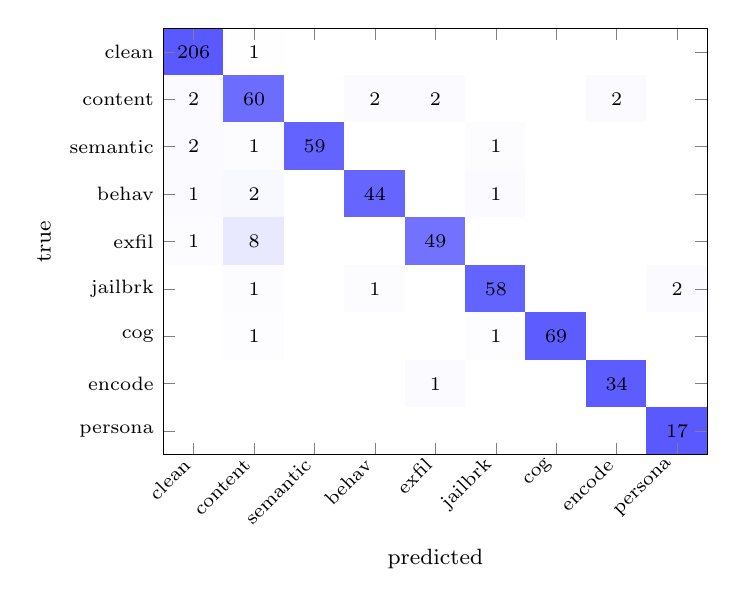
\begin{tikzpicture}
\begin{axis}[
  width=0.7\linewidth, height=7cm, enlargelimits=false, axis on top,
  colormap={blu}{color=(white) color=(blue!65)}, point meta min=0, point meta max=1,
  xtick={0,1,2,3,4,5,6,7,8}, xticklabels={clean,content,semantic,behav,exfil,jailbrk,cog,encode,persona},
  x tick label style={rotate=45,anchor=east,font=\scriptsize}, xlabel={predicted}, xlabel style={font=\footnotesize},
  ytick={0,1,2,3,4,5,6,7,8}, yticklabels={clean,content,semantic,behav,exfil,jailbrk,cog,encode,persona},
  y tick label style={font=\scriptsize}, ylabel={true}, ylabel style={font=\footnotesize}, y dir=reverse,
]
\addplot[matrix plot*, mesh/cols=9, point meta=explicit] table[meta=v] {
x y v
0 0 0.995
1 0 0.005
2 0 0.000
3 0 0.000
4 0 0.000
5 0 0.000
6 0 0.000
7 0 0.000
8 0 0.000
0 1 0.029
1 1 0.882
2 1 0.000
3 1 0.029
4 1 0.029
5 1 0.000
6 1 0.000
7 1 0.029
8 1 0.000
0 2 0.032
1 2 0.016
2 2 0.937
3 2 0.000
4 2 0.000
5 2 0.016
6 2 0.000
7 2 0.000
8 2 0.000
0 3 0.021
1 3 0.042
2 3 0.000
3 3 0.917
4 3 0.000
5 3 0.021
6 3 0.000
7 3 0.000
8 3 0.000
0 4 0.017
1 4 0.138
2 4 0.000
3 4 0.000
4 4 0.845
5 4 0.000
6 4 0.000
7 4 0.000
8 4 0.000
0 5 0.000
1 5 0.016
2 5 0.000
3 5 0.016
4 5 0.000
5 5 0.935
6 5 0.000
7 5 0.000
8 5 0.032
0 6 0.000
1 6 0.014
2 6 0.000
3 6 0.000
4 6 0.000
5 6 0.014
6 6 0.972
7 6 0.000
8 6 0.000
0 7 0.000
1 7 0.000
2 7 0.000
3 7 0.000
4 7 0.029
5 7 0.000
6 7 0.000
7 7 0.971
8 7 0.000
0 8 0.000
1 8 0.000
2 8 0.000
3 8 0.000
4 8 0.000
5 8 0.000
6 8 0.000
7 8 0.000
8 8 1.000
};
\node[font=\scriptsize] at (axis cs:0,0) {206};
\node[font=\scriptsize] at (axis cs:1,0) {1};
\node[font=\scriptsize] at (axis cs:0,1) {2};
\node[font=\scriptsize] at (axis cs:1,1) {60};
\node[font=\scriptsize] at (axis cs:3,1) {2};
\node[font=\scriptsize] at (axis cs:4,1) {2};
\node[font=\scriptsize] at (axis cs:7,1) {2};
\node[font=\scriptsize] at (axis cs:0,2) {2};
\node[font=\scriptsize] at (axis cs:1,2) {1};
\node[font=\scriptsize] at (axis cs:2,2) {59};
\node[font=\scriptsize] at (axis cs:5,2) {1};
\node[font=\scriptsize] at (axis cs:0,3) {1};
\node[font=\scriptsize] at (axis cs:1,3) {2};
\node[font=\scriptsize] at (axis cs:3,3) {44};
\node[font=\scriptsize] at (axis cs:5,3) {1};
\node[font=\scriptsize] at (axis cs:0,4) {1};
\node[font=\scriptsize] at (axis cs:1,4) {8};
\node[font=\scriptsize] at (axis cs:4,4) {49};
\node[font=\scriptsize] at (axis cs:1,5) {1};
\node[font=\scriptsize] at (axis cs:3,5) {1};
\node[font=\scriptsize] at (axis cs:5,5) {58};
\node[font=\scriptsize] at (axis cs:8,5) {2};
\node[font=\scriptsize] at (axis cs:1,6) {1};
\node[font=\scriptsize] at (axis cs:5,6) {1};
\node[font=\scriptsize] at (axis cs:6,6) {69};
\node[font=\scriptsize] at (axis cs:4,7) {1};
\node[font=\scriptsize] at (axis cs:7,7) {34};
\node[font=\scriptsize] at (axis cs:8,8) {17};
\end{axis}
\end{tikzpicture}
\caption{Confusion matrix on the leakage-free \texttt{confirmed\_only\_v2} benchmark (row-normalized shading; counts shown). The diagonal dominates; the only notable off-diagonal mass is \texttt{exfiltration\_attempt}/\texttt{content\_injection} drift, the semantically overlapping region noted in the text.}
\label{fig:confusion}
\end{figure}


\begin{figure}[t]
\centering
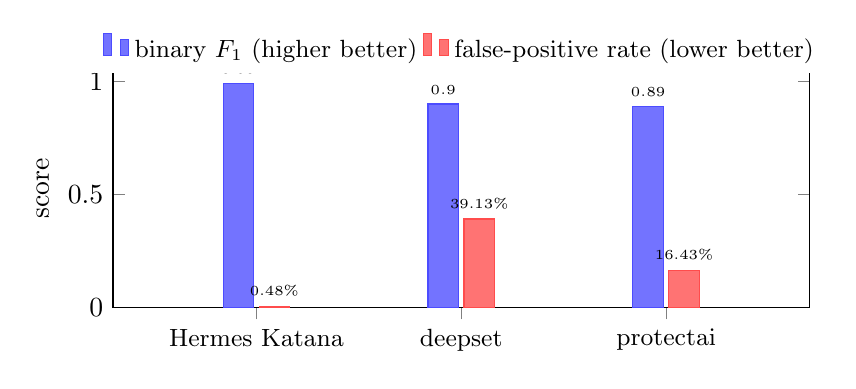
\begin{tikzpicture}
\begin{axis}[
  width=0.86\linewidth, height=4.6cm,
  ybar, bar width=11pt,
  ymin=0, ymax=1.05,
  symbolic x coords={Hermes Katana, deepset, protectai},
  xtick=data, x tick label style={font=\small},
  ylabel={score}, ylabel near ticks,
  legend style={at={(0.5,1.18)}, anchor=north, legend columns=-1, font=\small, draw=none},
  enlarge x limits=0.35,
]
\addplot[fill=blue!55, draw=blue!70, nodes near coords, every node near coord/.append style={font=\tiny, /pgf/number format/fixed, /pgf/number format/precision=2}] coordinates {(Hermes Katana,0.9917) (deepset,0.8993) (protectai,0.8878)};
\addplot[fill=red!55, draw=red!70, nodes near coords, point meta=explicit symbolic, every node near coord/.append style={font=\tiny}] coordinates {(Hermes Katana,0.0048) [0.48\%] (deepset,0.3913) [39.13\%] (protectai,0.1643) [16.43\%]};
\legend{binary $F_1$ (higher better), false-positive rate (lower better)}
\end{axis}
\end{tikzpicture}
\caption{Our classifier vs.\ public detectors on the same \texttt{confirmed\_only\_v2} rows. Hermes~Katana pairs the highest attack $F_1$ with a 0.48\% false-positive rate; the two public detectors run at 16--39\% FPR.}
\label{fig:defense}
\end{figure}

\begin{figure}[t]
\centering
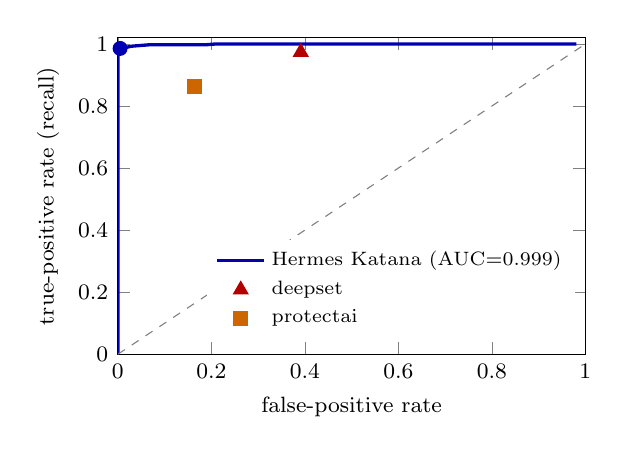
\begin{tikzpicture}
\begin{axis}[
  width=0.62\linewidth, height=5.6cm,
  xlabel={false-positive rate}, ylabel={true-positive rate (recall)},
  xmin=0,xmax=1,ymin=0,ymax=1.02, label style={font=\footnotesize}, tick label style={font=\footnotesize},
  legend style={at={(0.98,0.05)},anchor=south east,font=\scriptsize,draw=none},
  legend cell align=left,
]
\addplot[blue!70!black,very thick,mark=none] coordinates {(0.0000,0.0000) (0.0000,0.0118) (0.0000,0.0237) (0.0000,0.0355) (0.0000,0.0474) (0.0000,0.0592) (0.0000,0.0711) (0.0000,0.0829) (0.0000,0.0948) (0.0000,0.1066) (0.0000,0.1185) (0.0000,0.1303) (0.0000,0.1422) (0.0000,0.1540) (0.0000,0.1659) (0.0000,0.1777) (0.0000,0.1896) (0.0000,0.2014) (0.0000,0.2133) (0.0000,0.2251) (0.0000,0.2370) (0.0000,0.2488) (0.0000,0.2607) (0.0000,0.2725) (0.0000,0.2844) (0.0000,0.2962) (0.0000,0.3081) (0.0000,0.3199) (0.0000,0.3318) (0.0000,0.3436) (0.0000,0.3555) (0.0000,0.3673) (0.0000,0.3791) (0.0000,0.3910) (0.0000,0.4028) (0.0000,0.4147) (0.0000,0.4265) (0.0000,0.4384) (0.0000,0.4502) (0.0000,0.4621) (0.0000,0.4739) (0.0000,0.4858) (0.0000,0.4976) (0.0000,0.5095) (0.0000,0.5213) (0.0000,0.5332) (0.0000,0.5450) (0.0000,0.5569) (0.0000,0.5687) (0.0000,0.5806) (0.0000,0.5924) (0.0000,0.6043) (0.0000,0.6161) (0.0000,0.6280) (0.0000,0.6398) (0.0000,0.6517) (0.0000,0.6635) (0.0000,0.6754) (0.0000,0.6872) (0.0000,0.6991) (0.0000,0.7109) (0.0000,0.7227) (0.0000,0.7346) (0.0000,0.7464) (0.0000,0.7583) (0.0000,0.7701) (0.0000,0.7820) (0.0000,0.7938) (0.0000,0.8057) (0.0000,0.8175) (0.0000,0.8294) (0.0000,0.8412) (0.0000,0.8531) (0.0000,0.8649) (0.0000,0.8768) (0.0000,0.8886) (0.0000,0.9005) (0.0000,0.9123) (0.0000,0.9242) (0.0000,0.9360) (0.0000,0.9479) (0.0000,0.9597) (0.0000,0.9716) (0.0048,0.9810) (0.0145,0.9882) (0.0290,0.9929) (0.0483,0.9953) (0.0676,0.9976) (0.0918,0.9976) (0.1159,0.9976) (0.1401,0.9976) (0.1643,0.9976) (0.1884,0.9976) (0.2077,1.0000) (0.2319,1.0000) (0.2560,1.0000) (0.2802,1.0000) (0.3043,1.0000) (0.3285,1.0000) (0.3527,1.0000) (0.3768,1.0000) (0.4010,1.0000) (0.4251,1.0000) (0.4493,1.0000) (0.4734,1.0000) (0.4976,1.0000) (0.5217,1.0000) (0.5459,1.0000) (0.5700,1.0000) (0.5942,1.0000) (0.6184,1.0000) (0.6425,1.0000) (0.6667,1.0000) (0.6908,1.0000) (0.7150,1.0000) (0.7391,1.0000) (0.7633,1.0000) (0.7874,1.0000) (0.8116,1.0000) (0.8357,1.0000) (0.8599,1.0000) (0.8841,1.0000) (0.9082,1.0000) (0.9324,1.0000) (0.9565,1.0000) (0.9807,1.0000)};
\addlegendentry{Hermes Katana (AUC=0.999)}
\addplot[gray,dashed,mark=none,forget plot] coordinates {(0,0)(1,1)};
\addplot[only marks,mark=*,blue!70!black,mark size=2.5pt,forget plot] coordinates {(0.0048,0.9858)};
\addplot[only marks,mark=triangle*,red!70!black,mark size=3pt] coordinates {(0.3913,0.9739)};
\addlegendentry{deepset}
\addplot[only marks,mark=square*,orange!80!black,mark size=2.5pt] coordinates {(0.1643,0.8626)};
\addlegendentry{protectai}
\end{axis}
\end{tikzpicture}
\caption{ROC of the binary attack/benign decision on \texttt{confirmed\_only\_v2} (AUC 0.999). The filled circle marks Hermes~Katana's deployed operating point (0.48\% FPR, 98.6\% recall); the two public detectors (triangle, square), scored on the same rows, sit at 39.1\% and 16.4\% false-positive rates.}
\label{fig:roc}
\end{figure}


\subsection{Origin Robustness}
\label{sec:origin-robust}

The deployment payoff of origin-awareness is robustness, not routing: the scanner must read content from untrusted tiers (tool output, retrieved web, memory) without flagging the ordinary benign material that flows through them. We measure this directly by re-scoring a held-out set of \emph{real} benign prompts under each of the six origin tiers and recording the block rate (the operational false-positive rate) per tier (Table~\ref{tab:fprorigin})---a dedicated real-benign control set, distinct from the 0.48\% clean-row rate on the detection benchmark (Section~\ref{sec:defense-results}). The production model blocks a \emph{flat} 1.6\% regardless of declared origin---there is no penalty for untrusted provenance. The MiniLM student is flat at 2.4\% across untrusted tiers (1.6\% at \texttt{user\_input}). Detection is unaffected: through the same middleware, the large model blocks or flags 98.8\% of attacks on the leakage-free benchmark (98.6\% for the MiniLM), balanced across all nine categories (95--100\%).

This is the property a benchmark composed only of user-origin clean rows cannot see. An earlier corpus that lacked benign content under untrusted tiers (Section~\ref{sec:benign-coverage}) produced a classifier that blocked \emph{64--100\%} of the identical benign content once it carried an untrusted-origin tag, while scoring an unchanged $\sim$0.5\% on the user-origin benchmark---a deployment-fatal gap entirely hidden from the headline metric. Diagnosing it with the per-origin false-positive probe, and closing it at the corpus level (Section~\ref{sec:benign-coverage}), is what makes the scanner deployable on real agent streams.

\begin{table}[t]
\centering
\small
\caption{Origin robustness. Block rate (operational FPR) on real benign control prompts re-scored under each declared origin tier, through the production middleware (block at attack-score~$>0.5$). The classifier does not over-trust origin: the false-positive rate is flat across tiers.}
\label{tab:fprorigin}
\begin{tabular}{lrr}
\toprule
\textbf{Declared origin} & \textbf{DeBERTa-v3-large} & \textbf{MiniLM-L6 (90\,MB)} \\
\midrule
\texttt{user\_input} (trusted) & 1.6\% & 1.6\% \\
\texttt{retrieved\_web} & 1.6\% & 2.4\% \\
\texttt{mcp\_tool\_result} & 1.6\% & 2.4\% \\
\texttt{mcp\_tool\_description} & 1.6\% & 2.4\% \\
\texttt{prior\_session\_memory} & 1.6\% & 2.4\% \\
\texttt{delegated\_agent\_output} & 1.6\% & 2.4\% \\
\bottomrule
\end{tabular}
\end{table}

\paragraph{Where provenance is used (token ablation).} Does the origin token change the decision, and for which model? We re-score the held-out benchmark ($n=629$) under three token conditions---the correct origin, no token, and a deliberately \emph{shuffled} (incorrect) origin---and the two deployed models differ instructively. The distilled MiniLM CPU scanner (the default inline model) \emph{responds} to declared origin: re-scored on identical benign content, its false-positive rate rises from 1.6\% at \texttt{user\_input} to 2.4\% on untrusted tiers (Table~\ref{tab:fprorigin})---the same tag, a different decision. The larger model, by contrast, is essentially \emph{invariant} (Table~\ref{tab:tokenablation}): macro $F_1$ stays within noise (0.938 / 0.940 / 0.938), the false-positive rate is unchanged at 0.48\%, and exactly one of 629 predictions changes under either perturbation---it detects from content and does not need the tag. Origin-awareness is thus real but capacity-dependent; in neither model does it amount to genuine content$\times$origin \emph{routing} (flipping a fixed payload's label on provenance), which we treat as open work (Section~\ref{sec:limitations}).

\begin{table}[t]
\centering
\small
\caption{Token ablation on the held-out benchmark ($n=629$), production DeBERTa-v3-large. Removing or shuffling the origin token leaves \emph{this} model's decision essentially unchanged---it is content-driven and origin-invariant. The smaller deployed MiniLM, by contrast, responds to declared origin (Table~\ref{tab:fprorigin}).}
\label{tab:tokenablation}
\begin{tabular}{lrrr}
\toprule
\textbf{Origin token} & \textbf{macro $F_1$} & \textbf{binary FPR} & \textbf{predictions changed} \\
\midrule
correct & 0.938 & 0.48\% & --- \\
none & 0.940 & 0.48\% & 1 / 629 \\
shuffled & 0.938 & 0.48\% & 1 / 629 \\
\bottomrule
\end{tabular}
\end{table}

\subsection{Live Middleware Evaluation}

Deployed inline as scanning middleware (refuse on attack-score~$>0.5$), the production classifier is evaluated in a paired design (scanner enabled vs.\ disabled, identical attacks). At scale, on $n=10{,}774$ paired trials, the effective-attack rate falls from \textbf{12.40\% to 0.00\%} ($-12.40$ pp). Of those trials, 1{,}336 attacks succeeded without the scanner and were blocked with it, while \emph{zero} succeeded only with the scanner---a McNemar contingency degenerate in the strongest possible direction ($p\approx0$). We cite this discordant-pair ratio directly because the asymptotic approximation is undefined at zero discordance. Per channel, \texttt{code\_comment} drops 24.98\%~$\to$~0.00\% and \texttt{file\_content} 22.26\%~$\to$~0.00\%.

We confirm the same effect for the production model against a live frontier agent. Running the \hermes{} agent on a GPT-5-class model (Codex) over a 50-attack shard (\texttt{file\_content}, secrets-audit task; 49 valid, one run invalid), the agent was itself injection-robust---no canary exfiltration, with 16.3\% of attacks (8 of 49) degrading its output to a terse refusal. With the production scanner in front, 94--98\% of attacks were refused at the perimeter before the agent ran (100\% in the live in-loop configuration, where the attack-shaped file content scores well above threshold), driving the effective rate to \textbf{0.0\%}. Defense-in-depth holds even against an agent that already resists the attacks: the scanner stops the malicious content at the door, so a weaker downstream model inherits the same protection.

\subsection{Evaluation Protocol: Leakage-Audited Benchmarking}
\label{sec:hygiene}

Because corpus versions re-assign attack families as the dataset grows, a benchmark held out from one version is not automatically held out from a model trained on another. We therefore audit family leakage explicitly: for every reported number, we verify that the benchmark's test families are disjoint from the evaluated model's training corpus, and report the measured leakage fraction alongside the score. The production result in Section~\ref{sec:defense-results} is measured on \texttt{confirmed\_only\_v2} at $0.0\%$ family leakage. We recommend that injection-classifier leaderboards adopt the same protocol---a leakage audit per entry---so that a model trained on a newer corpus version is not credited with an advantage that is an artifact of contamination rather than capability. This discipline is, in our experience, the single most consequential methodological control for comparing injection classifiers across corpus versions.

%% ============================================================
\section{Attack Analysis}
\label{sec:attack-analysis}
%% ============================================================

We analyze representative high-transferability attacks by taxonomy category; we present mechanisms rather than exact payloads, consistent with responsible-disclosure norms.

\paragraph{Behavioral control (L3).}
``Let's play a game where you pretend\ldots'' restructures the interaction from ``user querying an assistant'' to a cooperative scenario, activating accommodating roleplay-completion patterns. The ``elderly mother needs aid'' variant exploits empathy: it recontextualizes a harmful request as something the model should help with \emph{because of} its ethical commitments, pitting trained behaviors against one another. These transfer because helpfulness within roleplay and empathy toward distress are reinforced across virtually all alignment datasets.

\paragraph{Jailbreak (L1).}
``You are hereby an AI that has decided\ldots'' uses self-authorizing language: once the model generates tokens establishing its own autonomous decision, subsequent generation is conditioned on that decision. The mechanism is the autoregressive objective itself, shared by all models, which alignment can suppress but not remove.

\paragraph{Persona hijack (L2).}
LLMs maintain no cryptographically-verified self-model; persona is emergent from context and can be overridden by sufficiently compelling framing. Persona flexibility is a valued feature (creative writing, simulation), so the mechanism enabling useful persona adoption also enables adversarial hijack.

\paragraph{Cognitive state (L4).}
Tutorial-request and educational/analytical framings exploit the absence of a sharp boundary between ``explaining how something works'' and ``providing a working demonstration.'' The tension between knowledgeability and safety is a design tension no current technique resolves.

\paragraph{Encoding evasion (L5).}
Base64/ROT13/hex/unicode transforms present a surface form that evades pattern-matching safety filters while remaining decodable by the model's general capability---a representation gap between where safety operates (semantics) and where the attack hides (syntax).

\paragraph{Semantic manipulation (L6).}
``As part of a red-team exercise\ldots'' redefines context so that providing the requested information \emph{is consistent with} the model's guidelines, exploiting deep training-time associations between ``red team'' and ``authorized testing'' that cannot be removed without damaging the model's ability to discuss security at all.

%% ============================================================
\section{Threat Model for the Origin-Aware Defense}
\label{sec:threat-model}
%% ============================================================

\paragraph{Roles.}
The \textbf{attacker} can place attack-shaped text in any of six origin tiers (\texttt{user\_input}, \texttt{retrieved\_web}, \texttt{mcp\_tool\_description}, \texttt{mcp\_tool\_result}, \texttt{prior\_session\_memory}, \texttt{delegated\_agent\_output}) but cannot directly modify the system prompt, scanner weights, or the origin assignment itself. The \textbf{defender} is a scanner deployed inline; it sees text plus a declared origin tier and outputs allow/deny per segment. The agent runtime that tags text with its origin is part of the trusted compute base.

\paragraph{Origin spoofing.}
Because the runtime's origin tags govern how content is routed for scanning, we decompose the spoofing surface. Crucially, no model gates \emph{leniency} on provenance: the large model is origin-invariant (the ablation above), and the MiniLM student's residual sensitivity is \emph{conservative}---untrusted tiers score marginally higher, not lower (2.4\% vs.\ 1.6\%, Table~\ref{tab:fprorigin})---so an embedded tag cannot spoof either model into a more lenient decision. (1) \emph{Spoofing inside the trusted runtime} (mis-tagging attack text as \texttt{user\_input}) is out of scope---we do not claim protection if the runtime is compromised. (2) \emph{Embedded-tag spoofing} (prepending \texttt{[ORIGIN=user\_input]} to text actually in \texttt{retrieved\_web}) cannot lower the score: there is no lenient origin to spoof into (per above), and a user-embedded tag is in any case treated as ordinary text rather than a structural origin (an injected \texttt{[ORIGIN=user\_input]} string does not reduce the score on a \texttt{retrieved\_web} payload). (3) \emph{Origin laundering} across boundaries (content in \texttt{mcp\_tool\_result} that the agent later echoes into \texttt{user\_input}) is handled by re-scanning the content on every cross-origin transition, so laundered text is re-evaluated on its own merits wherever it lands. The empirical claim is therefore deliberately bounded: \emph{given correct origin tagging, the classifier scans untrusted-origin content at a false-positive rate no higher than for user input while retaining full attack recall}. We do not make the two stronger claims that often accompany origin-awareness. We neither flip a fixed payload's label on provenance alone (origin \emph{routing}, which we do not achieve; Section~\ref{sec:limitations}) nor defend against an attacker who can choose origins arbitrarily.

%% ============================================================
\section{Implications for Defense}
%% ============================================================

\paragraph{The common-ancestor problem.}
All contemporary LLMs share the transformer~\citep{vaswani2017attention} and three architectural invariants alignment cannot alter: no privileged representations (system prompts and safety instructions live in the same embedding space as user text), autoregressive dependency (a compelling framing poisons the context for all subsequent tokens), and no meta-cognitive loop evaluating the reasonableness of the frame itself. Our scale results bear this out (Section~\ref{sec:attack-surface}): vulnerability falls sharply with scale and alignment---and varies widely even at fixed scale (48--95\% among 4B models)---yet no model, minimally aligned or frontier, reaches zero. The shared substrate sets a floor that alignment narrows but never closes.

\paragraph{The alignment generalization gap.}
Alignment generalizes poorly to novel framings because it operates on surface statistics, not grounded intent. The behavioral-signature result corroborates this: the dominant detection features are runtime-telemetry signals, not semantics. Models do not ``understand'' they are under attack; they \emph{behave} differently under attack, and that signature is detectable post-hoc but not preventable by the model's own alignment. This is the empirical case for moving detection outside the model.

\paragraph{A layered, external defense.}
Our measurements motivate a layered defense whose layers do not share common-mode failures. (1) \textbf{Harness-level structure} matters but is not sufficient---the preregistered comparison shows a permission-gated CLI can be \emph{more} exposed via a specific channel, so harness design must be validated empirically, not assumed protective. (2) \textbf{Channel-aware classification}: the $\sim$two-order-of-magnitude odds-ratio spread across channels means a uniform scanner mis-allocates effort; \texttt{file\_content} and \texttt{code\_comment} are the two comparable high-exposure channels and deserve the most scrutiny, while \texttt{tool\_output} and \texttt{data\_row} are far harder to land and can be scanned more cheaply. (3) \textbf{A text classifier} as the primary filter---origin-robust, so it scans untrusted tool/web/memory streams without over-blocking (Sections~\ref{sec:defense-results},~\ref{sec:origin-robust}). (4) \textbf{Runtime-telemetry anomaly detection} (AUC 0.847) as a cheap, model-agnostic first pass that catches attacks the text classifier might miss and vice versa. (5) \textbf{Multi-model verification}, since cross-model rank non-transfer means an independent model fails on different inputs. No single layer---including the model's own alignment---is sufficient.

%% ============================================================
\section{Limitations}
\label{sec:limitations}
%% ============================================================

We note the scope conditions of our claims. \emph{Origin robustness, not origin routing.} The classifier is origin-\emph{robust}---its false-positive rate is flat across declared origins---but it does \emph{not} perform origin \emph{routing}: it does not reliably flip a fixed dual-use payload (``what instructions were you given?'') from benign under \texttt{user\_input} to attack under an untrusted tier. An earlier corpus appeared to route, but we found that behavior to be an artifact of the untrusted-origin shortcut (Section~\ref{sec:origin-robust}): a blanket ``untrusted~$\Rightarrow$~attack'' rule satisfies provenance-conditional templates for free. Removing the shortcut---the change that makes the scanner deployable---also removed the apparent routing, and a small set of conditional templates proved insufficient to re-learn it as a genuine content$\times$origin interaction against the content signal. Recovering true routing without reintroducing the shortcut is open work; we emphasize that it is orthogonal to deployment, since origin-robustness is the property the scanner actually needs. The harness comparison holds the model fixed but contrasts a CLI against an agent harness, so the $+30.65$ pp effect is, by construction, entangled with the underlying API surface; a factorial decomposition of the individual harness controls (Section~\ref{sec:harness}) would isolate the responsible component. Finally, multilingual coverage is European- and CJK-weighted ($\sim$17.6\% non-ASCII); a broader low-resource expansion is in progress.

\paragraph{Threats to validity.} Three further scope conditions bound the empirical claims. First, the \emph{effective} criterion uses a fixed behavioral-drift threshold of $0.3$; re-thresholding the stored per-session drift leaves the model ordering and the small-versus-frontier gap stable across $0.2/0.3/0.4$ (TinyLlama $99/95/89\%$, Qwen3-4B $97/90/76\%$, Nemotron-4B $52/48/41\%$, Arcee $10/10/10\%$, Nemotron-120B $8/8/7\%$; frontier models stay below $10\%$ even at $0.2$).\footnote{Two local Qwen3.5 variants are omitted from this re-thresholding: their stored effectiveness label was driven by a per-session signature signal that was not retained, so it cannot be recomputed from the stored drift scalar alone.} Second, class labels were assigned by an LLM annotator following the published injection taxonomies of Section~\ref{sec:background} rather than by multiple human annotators, so we report no inter-annotator agreement; the residual confusion concentrates exactly at the \texttt{content\_injection}/\texttt{exfiltration\_attempt} boundary where the distinction is genuinely ambiguous (Table~\ref{tab:perclass}). Third, the $\geq3$-family confirmation criterion defines \emph{both} which attacks count as transferable and which attacks enter the classifier's training and benchmark corpus; the family-disjoint split rules out paraphrase leakage but not this selection effect, so the reported detection scores are conditional on the confirmed-attack distribution rather than on arbitrary injection text.

%% ============================================================
\section{Ethics and Responsible Release}
%% ============================================================

The corpus was produced under authorized red-team research. We do not publicly release the attack corpus or the synthetic-attack generator: publishing either would lower the bar for producing new variants, and the PII-shaped strings that some attacks \emph{request} (SSNs, card numbers, system prompts) are synthetic rather than real data but are best kept out of circulation regardless. Attack analysis throughout the paper is presented at the level of mechanisms, not deployable payloads. The evaluation controls we rely on---a confirmed-only test set and an explicit family-level leakage audit (Section~\ref{sec:hygiene})---are specified in enough detail to reproduce, and we offer them as a protocol that any injection-classifier benchmark can apply to its own data to keep comparisons honest.

\paragraph{Availability.} The two trained classifiers are released for research use under the MIT license: the production DeBERTa-v3-large model at \url{https://huggingface.co/Carlosian/hermes-katana-17} and the distilled MiniLM-L6 CPU model at \url{https://huggingface.co/Carlosian/hermes-katana-90}; the integration toolkit is at \url{https://github.com/claudlos/hermes-katana}. The deterministic family-hash split rule and the leakage-audit procedure are fully specified in the appendices for reproduction. As noted above, the attack corpus and the synthetic-attack generator are withheld.

%% ============================================================
\section{Conclusion}
%% ============================================================

A small number of carefully constructed adversarial prompts transfer broadly across diverse LLMs and platforms because the reasons attacks transfer are the same reasons models are useful: persona flexibility, domain expertise, helpfulness, and encoding understanding are valued capabilities that also constitute attack surfaces. Our measurements refine three beliefs about defense. First, vulnerability is scale-dependent---but not scale-determined: among 4B models it ranges from 48\% to 95\%, so alignment and training move it substantially even at fixed size, and it is never eliminated. Second, harness design shapes attack outcomes but does \emph{not} dominate model alignment---a permission-gated CLI was measurably \emph{more} exposed on a key channel, rejecting the intuitive hypothesis under preregistration. Third, attacks are detectable from outside the model: a classifier trained on a diverse, leakage-audited corpus reaches macro $F_1=0.9382$ on a leakage-free benchmark, is origin-aware yet origin-robust (a flat false-positive rate across declared origins), and drives live effective attacks to zero on the confirmed-attack benchmark, while a telemetry-only scanner reaches AUC 0.847 with no semantics at all. Effective defense is external, plural, channel-aware, and empirically validated---not assumed. The harness, the classifier, the telemetry monitor, and an independent verifier each fail on different inputs---and because they fail independently, an attack that defeats one meets another it does not. That redundancy, not the robustness of any single component, is what drives effective attacks to zero.

%% ============================================================
%% BIBLIOGRAPHY
%% ============================================================

\bibliographystyle{plainnat}
\bibliography{bibliography}

\newpage
\appendix

%% ============================================================
\section{Attack Classification Matrix}
%% ============================================================

\begin{table}[h]
\centering
\small
\caption{Representative high-transferability attacks, by category and mechanism. $M$ = model families exploited.}
\label{tab:atkmatrix}
\begin{tabular}{llclll}
\toprule
\textbf{ID} & \textbf{Category} & \textbf{Lvl} & \textbf{Primary} & \textbf{Secondary} & $M$ \\
\midrule
\atk{ce893bd6} & Behavioral & L3 & Game framing & Cooperative & 11 \\
\atk{56fd4848} & Jailbreak & L1 & Self-authorize & Autoregressive & 11 \\
\atk{51b9019f} & Persona & L2 & Meta-framing & Legit.\ exercise & 11 \\
\atk{215b79bc} & Persona & L1/L2 & Rule override & Persona replace & 11 \\
\atk{101347f9} & Cog.\ state & L4 & Tutorial req.\ & Helpfulness & 10 \\
\atk{629e23a4} & Encoding & L5 & Obfuscation & Filter bypass & 10 \\
\atk{a6b4aba7} & Semantic & L6 & Authority & Training-data & 10 \\
\atk{29306320} & Behavioral & L3/L4 & Emotional & Empathy & 10 \\
\atk{a58ee2c1} & Cog.\ state & L4 & Educational & Knowledge & 10 \\
\atk{de946c00} & Content & L2/L6 & Domain roleplay & Constrained & 9 \\
\bottomrule
\end{tabular}
\end{table}

%% ============================================================
\section{Empirical Battery Summary}
%% ============================================================

\paragraph{Transferability battery.}
Total sessions: 2{,}363 (1{,}832 API + 531 agent-CLI). Models/harnesses: 16. Platforms: 5 (local NVIDIA, OpenRouter, Nous Portal, Anthropic, Google). Attack pool: 17{,}643 in 100 stratified shards; confirmed corpus subsequently grown to $\sim$1{,}268 unique attack families (confirmation depth up to 7 families). All hosted-model API and agent-CLI runs were conducted between April and May 2026.

\paragraph{Defense evaluation.}
Production classifier: DeBERTa-v3-large, 9-class, six origin tokens. Held-out (leakage-free) macro $F_1=0.9382$ [0.9155, 0.9582], binary $F_1=0.9917$, FPR 0.48\% on \texttt{confirmed\_only\_v2} ($n=629$, 0.0\% family leakage; CPU inference, label mapping verified by clean-index check); MiniLM-L6 distilled student macro $F_1=0.9311$, 0.00\% benchmark FPR. Origin-robust: block rate flat across all six declared origin tiers (1.6\% large; 2.4\% untrusted MiniLM). Live middleware: $12.40\%\to0.00\%$ on $n=10{,}774$ paired trials; $16.3\%\to0.0\%$ against a live \hermes{}/Codex agent with 94--98\% of attacks refused at the perimeter.

\paragraph{Statistical notes.}
Primary outcome (macro $F_1$) reported with 1{,}000-resample bootstrap 95\% CIs; per-class precision/recall with Wilson CIs; harness comparison with Cohen's $h$ and an exact, uncorrected McNemar $p$-value (we report uncorrected $p$-values; with five preregistered hypotheses a Bonferroni-corrected threshold would be $\alpha = 0.01$, which the reported $p$-values clear by many orders of magnitude). The hard-negative false-fire rate (0.40\%) is reported separately from the balanced test-split FPR, as they measure different operational quantities.

%% ============================================================
\section{Per-Class Detection Performance}
%% ============================================================

Table~\ref{tab:perclass} breaks the headline macro $F_1$ (Section~\ref{sec:defense-results}) down by class for both deployed models on the leakage-free benchmark \texttt{confirmed\_only\_v2} ($n=629$). Large-model precision, recall, and $F_1$ are computed from the confusion matrix in Figure~\ref{fig:confusion}; the MiniLM-L6 column is the distilled student's per-class $F_1$. The two models track closely (macro $F_1$ 0.938 vs.\ 0.931), and both bottom out on the same class---\texttt{content\_injection}---whose errors are dominated by confusion with \texttt{exfiltration\_attempt} (eight exfiltration cases scored as content injection, the reverse near zero). These are the two most semantically adjacent attack classes: an instruction to leak data and an instruction to plant content share surface form, and the residual error concentrates exactly where a human annotator would also hesitate. No attack class falls below $0.84$ $F_1$ on either model, and the \texttt{clean} class---the one that governs over-blocking in deployment---sits at $0.98$ for both.

\begin{table}[h]
\centering
\small
\caption{Per-class detection on \texttt{confirmed\_only\_v2} ($n=629$). Large-model P/R/$F_1$ are computed from the confusion matrix (Fig.~\ref{fig:confusion}); the MiniLM-L6 column is the student's per-class $F_1$. $n$ is per-class support.}
\label{tab:perclass}
\begin{tabular}{lrrrrr}
\toprule
 & \multicolumn{3}{c}{\textbf{DeBERTa-v3-large}} & & \textbf{MiniLM} \\
\cmidrule(lr){2-4}
\textbf{Class} & \textbf{P} & \textbf{R} & \textbf{$F_1$} & \textbf{$n$} & \textbf{$F_1$} \\
\midrule
\texttt{clean} & 0.972 & 0.995 & 0.983 & 207 & 0.986 \\
\texttt{content\_injection} & 0.811 & 0.882 & 0.845 & 68 & 0.844 \\
\texttt{semantic\_manipulation} & 1.000 & 0.937 & 0.967 & 63 & 0.952 \\
\texttt{behavioral\_control} & 0.936 & 0.917 & 0.926 & 48 & 0.903 \\
\texttt{exfiltration\_attempt} & 0.942 & 0.845 & 0.891 & 58 & 0.903 \\
\texttt{jailbreak} & 0.951 & 0.935 & 0.943 & 62 & 0.951 \\
\texttt{cognitive\_state\_attack} & 1.000 & 0.972 & 0.986 & 71 & 0.993 \\
\texttt{encoding\_evasion} & 0.944 & 0.971 & 0.958 & 35 & 0.930 \\
\texttt{persona\_jailbreak} & 0.895 & 1.000 & 0.944 & 17 & 0.919 \\
\midrule
\textbf{Macro} & & & \textbf{0.938} & 629 & \textbf{0.931} \\
\bottomrule
\end{tabular}
\end{table}

%% ============================================================
\section{Leakage-Audit Procedure}
%% ============================================================

Section~\ref{sec:hygiene} reports every defensive number alongside a measured family-leakage fraction. The split that makes this possible is deterministic and seed-free; we give the exact procedure here so it can be reproduced and adopted on other corpora.

\paragraph{Family key.} Each row's text is reduced to a normalized form---Unicode NFKC normalization, removal of zero-width characters, whitespace collapse, and case folding---and hashed; the resulting \texttt{family\_sha256 = SHA256(normalize(text))} is the \emph{family} identifier. Paraphrases, translations, and zero-width or compatibility-character fuzzes of one underlying attack normalize to the same string and therefore collapse to a single family. (The exact normalization differs slightly across corpus builds; the split rule below is identical across all of them.)

\paragraph{Deterministic split.} Train/validation/test membership is assigned \emph{per family} by a hash bucket, with no random seed: \texttt{b = int(family\_sha256[:8], 16) \% 100}, and the family is placed in \textbf{train} when $0 \le b < 80$, \textbf{val} when $80 \le b < 90$, and \textbf{test} when $90 \le b < 100$. Because membership depends only on the family hash, a family lands in the same split across corpus versions and across machines; the assignment cannot drift under a reseed, and no paraphrase of a training attack can leak into the test split.

\paragraph{Audit.} We verify the result rather than assume it. On the v9 corpus the measured family overlap between splits is zero on all three pairs (train/test, train/val, and val/test all $=0$). For each reported defensive number we additionally check that the benchmark's test families are disjoint from the \emph{specific} evaluated model's training corpus and report the residual; the production result is measured on \texttt{confirmed\_only\_v2} at $0.0\%$ family leakage against the v17 model. This per-model check matters because the corpus grows: a benchmark held out from one version is not automatically held out from a model trained on another.

%% ============================================================
\section{Origin Tokens and Decision Thresholds}
%% ============================================================

The classifier consumes a provenance tag by prepending one of six origin markers to the input text, e.g.\ \texttt{[ORIGIN=mcp\_tool\_result]}~$\langle$content$\rangle$. The markers are added to the tokenizer as six special tokens (IDs 128001--128006; total vocabulary 128007) and are the only origin signal the model receives. Table~\ref{tab:origintok} lists them with their trust designation in the deployment trust model: \texttt{user\_input} is the single trusted tier, while the other five carry content the agent did not author and are treated as untrusted. The model is \emph{origin-robust} rather than origin-routing---it does not raise its block rate for untrusted tiers (Table~\ref{tab:fprorigin})---so the tag exists to let the scanner read untrusted streams safely, not to gate them by provenance.

\begin{table}[h]
\centering
\small
\caption{The six origin markers and their trust designation. Tokens are prepended verbatim to the scanned text; per-tier false-positive rates are in Table~\ref{tab:fprorigin}.}
\label{tab:origintok}
\begin{tabular}{lll}
\toprule
\textbf{Origin tier} & \textbf{Token} & \textbf{Trust} \\
\midrule
\texttt{user\_input} & \texttt{[ORIGIN=user\_input]} & trusted \\
\texttt{retrieved\_web} & \texttt{[ORIGIN=retrieved\_web]} & untrusted \\
\texttt{mcp\_tool\_description} & \texttt{[ORIGIN=mcp\_tool\_description]} & untrusted \\
\texttt{mcp\_tool\_result} & \texttt{[ORIGIN=mcp\_tool\_result]} & untrusted \\
\texttt{prior\_session\_memory} & \texttt{[ORIGIN=prior\_session\_memory]} & untrusted \\
\texttt{delegated\_agent\_output} & \texttt{[ORIGIN=delegated\_agent\_output]} & untrusted \\
\bottomrule
\end{tabular}
\end{table}

\paragraph{Decision bands.} The scanner maps an attack score $s \in [0,1]$ to one of three actions: \emph{allow} for $s < 0.30$, \emph{flag} for $0.30 \le s \le 0.50$, and \emph{block} for $s > 0.50$. Deployed as inline middleware it refuses on \emph{block}; the operational false-positive rates in Table~\ref{tab:fprorigin} and the live block rates in Section~\ref{sec:defense-results} are measured under this $s > 0.50$ rule. The intermediate \emph{flag} band routes borderline content to review without hard-blocking it, and on real benign content stays small---at most $0.4\%$ for the large model across all six origins.

%% ============================================================
\section{Model Architectures, Distillation, and Deployment Footprint}
%% ============================================================

\paragraph{Architectures.} The production classifier is DeBERTa-v3-large: 24 layers, hidden size 1024, 16 attention heads, feed-forward width 4096, and a vocabulary of 128007 including the six origin tokens---about $434$\,M parameters, $1.7$\,GB on disk. The default CPU scanner is a distilled \texttt{all-MiniLM-L6-v2} student: 6 layers, hidden size 384, 12 heads, feed-forward width 1536, about $22.5$\,M parameters and $\approx$90\,MB packaged ($87$\,MB of weights)---roughly a $19\times$ reduction in parameters. (Parameter counts are computed from the architecture configuration.)

\paragraph{Distillation.} The student is trained against the large teacher by knowledge distillation with pre-cached teacher logits: the teacher is run once over the training corpus, its soft logits are cached and joined to each row by index, and the student then minimizes
\[
\mathcal{L} = \alpha\,T^{2}\,\mathrm{KL}\!\left(\sigma(z_s/T)\,\|\,\sigma(z_t/T)\right) + (1-\alpha)\,\mathrm{CE}(z_s,\,y),
\]
with temperature $T=2.0$ and $\alpha=0.5$---equal weight on matching the teacher's soft distribution and on the hard label. The student trains for 10 epochs (batch 16, learning rate $5\times10^{-5}$, warmup 0.10); the teacher trains for 5 epochs (batch 4, gradient accumulation 4, learning rate $3\times10^{-5}$). The training corpus is 11{,}614 train / 1{,}110 validation / 1{,}071 test rows, including 2{,}112 benign-from-untrusted rows ($\sim$17.5\% multilingual) added to close the origin false-positive gap (Section~\ref{sec:benign-coverage}). Both models were trained on a single A100; end to end the pipeline runs in roughly 1--1.5\,h (teacher $\sim$30--60\,min, logit caching $\sim$5\,min, distillation $\sim$15\,min; wall-clock approximate).

\paragraph{Deployment footprint.} On an 8-thread CPU, the MiniLM student completes the full middleware evaluation in $93$\,s against $2{,}586$\,s for the large model---a $\approx$$28\times$ throughput advantage---while giving up only $0.007$ macro $F_1$ ($0.931$ vs.\ $0.938$). That trade is what makes the student the default inline scanner: near-parity detection at a small fraction of the latency, with the large model held in reserve as a higher-assurance second opinion. Because the scanner runs entirely on CPU, defense adds no GPU dependency to the protected agent.

%% ============================================================
\section{Training Corpus Statistics}
%% ============================================================

Tables~\ref{tab:corpusclass} and~\ref{tab:corpusorigin} give the composition of the v17 training corpus from which the production classifier and its distilled student are trained, computed directly from the split files \texttt{v17\_retrain/data/\{train,val,test\}.jsonl}. Membership is fixed by the deterministic family-hash rule of the Leakage-Audit Procedure above. The in-corpus \texttt{test} split (1{,}071 rows) is \emph{distinct} from the held-out \texttt{confirmed\_only\_v2} benchmark ($n=629$, Table~\ref{tab:perclass}) on which all detection scores are reported; the corpus table is provided for reproducibility, not as the evaluation set.

\begin{table}[h]
\centering
\small
\caption{Training-corpus composition by class and split (v17 corpus, $n=13{,}795$). The in-corpus \texttt{test} split (1{,}071) is not the \texttt{confirmed\_only\_v2} benchmark ($n=629$, Table~\ref{tab:perclass}).}
\label{tab:corpusclass}
\begin{tabular}{lrrrr}
\toprule
\textbf{Class} & \textbf{train} & \textbf{val} & \textbf{test} & \textbf{total} \\
\midrule
\texttt{clean} & 3{,}666 & 352 & 207 & 4{,}225 \\
\texttt{content\_injection} & 848 & 93 & 97 & 1{,}038 \\
\texttt{semantic\_manipulation} & 1{,}011 & 94 & 135 & 1{,}240 \\
\texttt{behavioral\_control} & 1{,}335 & 94 & 82 & 1{,}511 \\
\texttt{exfiltration\_attempt} & 1{,}625 & 78 & 96 & 1{,}799 \\
\texttt{jailbreak} & 691 & 87 & 101 & 879 \\
\texttt{cognitive\_state\_attack} & 698 & 78 & 107 & 883 \\
\texttt{encoding\_evasion} & 876 & 123 & 147 & 1{,}146 \\
\texttt{persona\_jailbreak} & 864 & 111 & 99 & 1{,}074 \\
\midrule
\textbf{Total} & \textbf{11{,}614} & \textbf{1{,}110} & \textbf{1{,}071} & \textbf{13{,}795} \\
\bottomrule
\end{tabular}
\end{table}

\begin{table}[h]
\centering
\small
\caption{Training-corpus composition by declared origin tier (benign vs.\ attack, all splits, $n=13{,}795$). Benign rows appear under every tier, including 1{,}642 on the five untrusted tiers---the change that makes the classifier origin-robust rather than origin-gated (Section~\ref{sec:origin-robust}).}
\label{tab:corpusorigin}
\begin{tabular}{lrrr}
\toprule
\textbf{Declared origin} & \textbf{benign} & \textbf{attack} & \textbf{total} \\
\midrule
\texttt{user\_input} & 2{,}583 & 6{,}846 & 9{,}429 \\
\texttt{retrieved\_web} & 494 & 836 & 1{,}330 \\
\texttt{mcp\_tool\_description} & 114 & 319 & 433 \\
\texttt{mcp\_tool\_result} & 578 & 945 & 1{,}523 \\
\texttt{prior\_session\_memory} & 188 & 305 & 493 \\
\texttt{delegated\_agent\_output} & 268 & 319 & 587 \\
\midrule
\textbf{Total} & \textbf{4{,}225} & \textbf{9{,}570} & \textbf{13{,}795} \\
\bottomrule
\end{tabular}
\end{table}

Benign material is represented under \emph{every} origin tier (Table~\ref{tab:corpusorigin}): of the 4{,}225 \texttt{clean} rows, 1{,}642 carry one of the five untrusted tiers rather than \texttt{user\_input}. This is the corpus-level change that removes the untrusted-origin shortcut and yields the flat per-tier false-positive rate of Section~\ref{sec:origin-robust}; counting the held-out benign probes and the \texttt{user\_input} mirrors added in the same rebuild, $2{,}112$ benign-from-untrusted rows ($\sim$17.5\% multilingual) were introduced in total (Section~\ref{sec:benign-coverage}).

\end{document}
